\subsection{Communication}
% communication
In total 11 groups used the built-in messaging tool and sent 341 messages. Most of the messages were sent outside class time, with a few sent in class simply to check if the tool functioned as expected. This is not surprising as typing messages costs more efforts if they could simply talk to each other face-to-face in class.

There are several reasons why other groups did not use the messaging tool. For example, some groups chose to work face-to-face all the time. They met together outside class. Some groups used other messaging tools, such as GroupMe \footnote{https://groupme.com/} and phone text. We imagine that they preferred those tools because they were more used to the tools and messages in those tools were immediately accessible through mobile phone. Finally, some groups mentioned that they felt no need to message because they had planned well beforehand in class. With the real time sharing of the system, they could put things together without further discussion.

% for messaging users, what did they talk?
For groups who used the messaging tool, their messages fell into these categories: 1) dividing work. This happened when coordinating writing the group report. The group had already had a clear understanding of the case and assigned members to write up different sections of the report. 2) clarifying task, such as what is the required submission of the project. 3) pointing teammates to other resources. Some groups might create documents outside the system, e.g. create a document in Google Doc 4) discussing hypotheses. Individuals could have different hypotheses on the same information. Sharing hypotheses and exploring related evidence helped develop the story. Figure \ref{tab:chat} is an example how groups collectively constructed a story. Previously their team tended to believe the suspect Redd was involved in all seven cases. S1 challenged the belief by bringing a piece of evidence he found. But S2 gave a possible explanation against the evidence. S1 continued to raise other evidence and won the support of S3. S1 then proposed another hypothesis that Redd might be only related to the last case. The team further collected and discussed related facts and eventually developed a theory including the suspect's motivation.


% group dialog example
\begin{table}
	\centering
	\caption{Group message excerpt}
    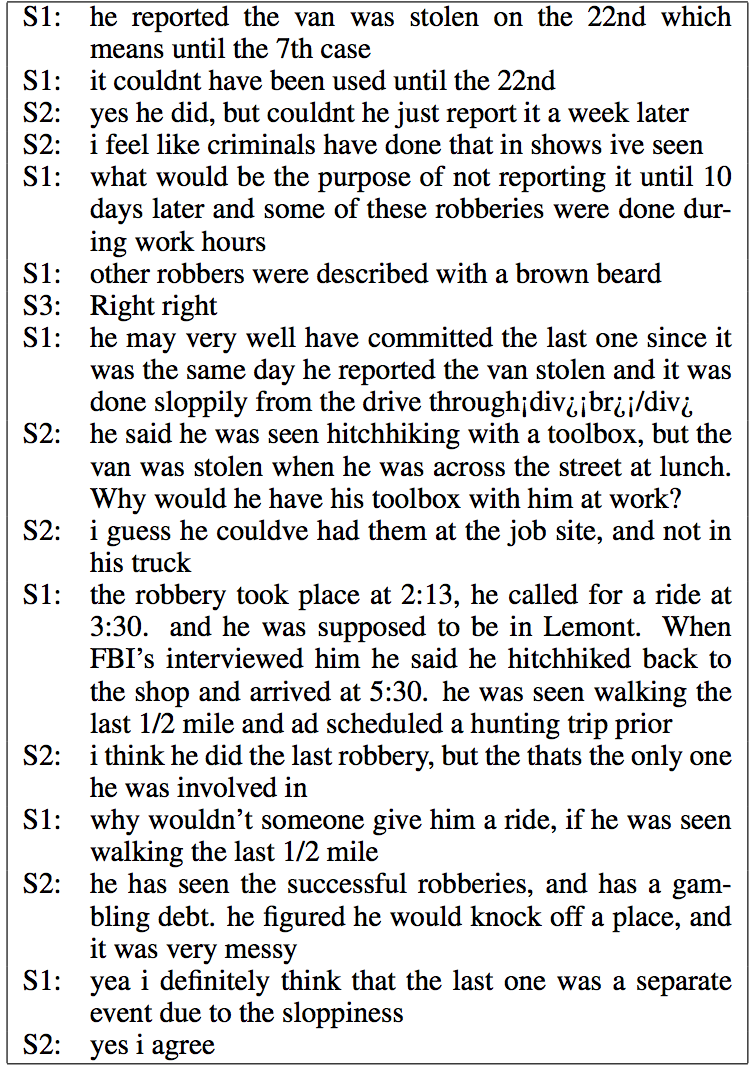
\includegraphics[width=.9\linewidth]{img/group_chat}
	\label{tab:chat}
\end{table}
% end group dialog

For groups who used the message tool, they believed it facilitated their communication, especially outside class. 
\textit{`I think what was different was the communication outside of class when we didn\'t have CAnalytics. Having a team member who works just about everyday, and living off campus makes the messaging very useful. Being able to message and reference things on the program made working outside of class a lot smoother rather than texting each other or finding a time that worked well with everyone.'}

% less time for constant check and clarify
\textit{`I think we communicated less because everyone could see what each other was working on immediately and therefore there was not a need to constantly update each other about what we were working on'.}


The function to refer to data objects in the system was not much used. One student mentioned he used the reference function to point to his teammates' attention of a data object. 
\textit{`When I agreed or disagreed with his annotations, I messaged him over the messenger tool to discuss our analysis'.}
 Another student also made a positive comment:
\textit{`Being able to add a link, for example, in the messaging system was very beneficial and worked almost as well as communicating in person'.}

% negative consequence of communication
In contrast, some students thought CAnalytics hindered their team communication. With traditional tools, teams were ``forced'' to constantly update what they found. Yet they felt CAnalytics created an illusion that little extra communication was necessary because everything was shared immediately. This, however, eventually hindered team communication.


\textit{`With the CAnalytics tool, we could observe each other’s work so there was technically no reason to talk with each other and it ultimately was not as effective in my opinion for group work.'}



